\chapter{Descripción del diseño de la base de datos}\label{chapter:database}

\section{Modelación de la asignación de docencia}
En la fase de diseño conceptual se modelaron las entidades fundamentales
que intervienen en el proceso de la asignación de docencia, 
así como las interrelaciones que se establecen entre ellas
y se obtuvo el siguiente
esquema a partir del modelo entidad-relación extendido.

\begin{figure}[H]
    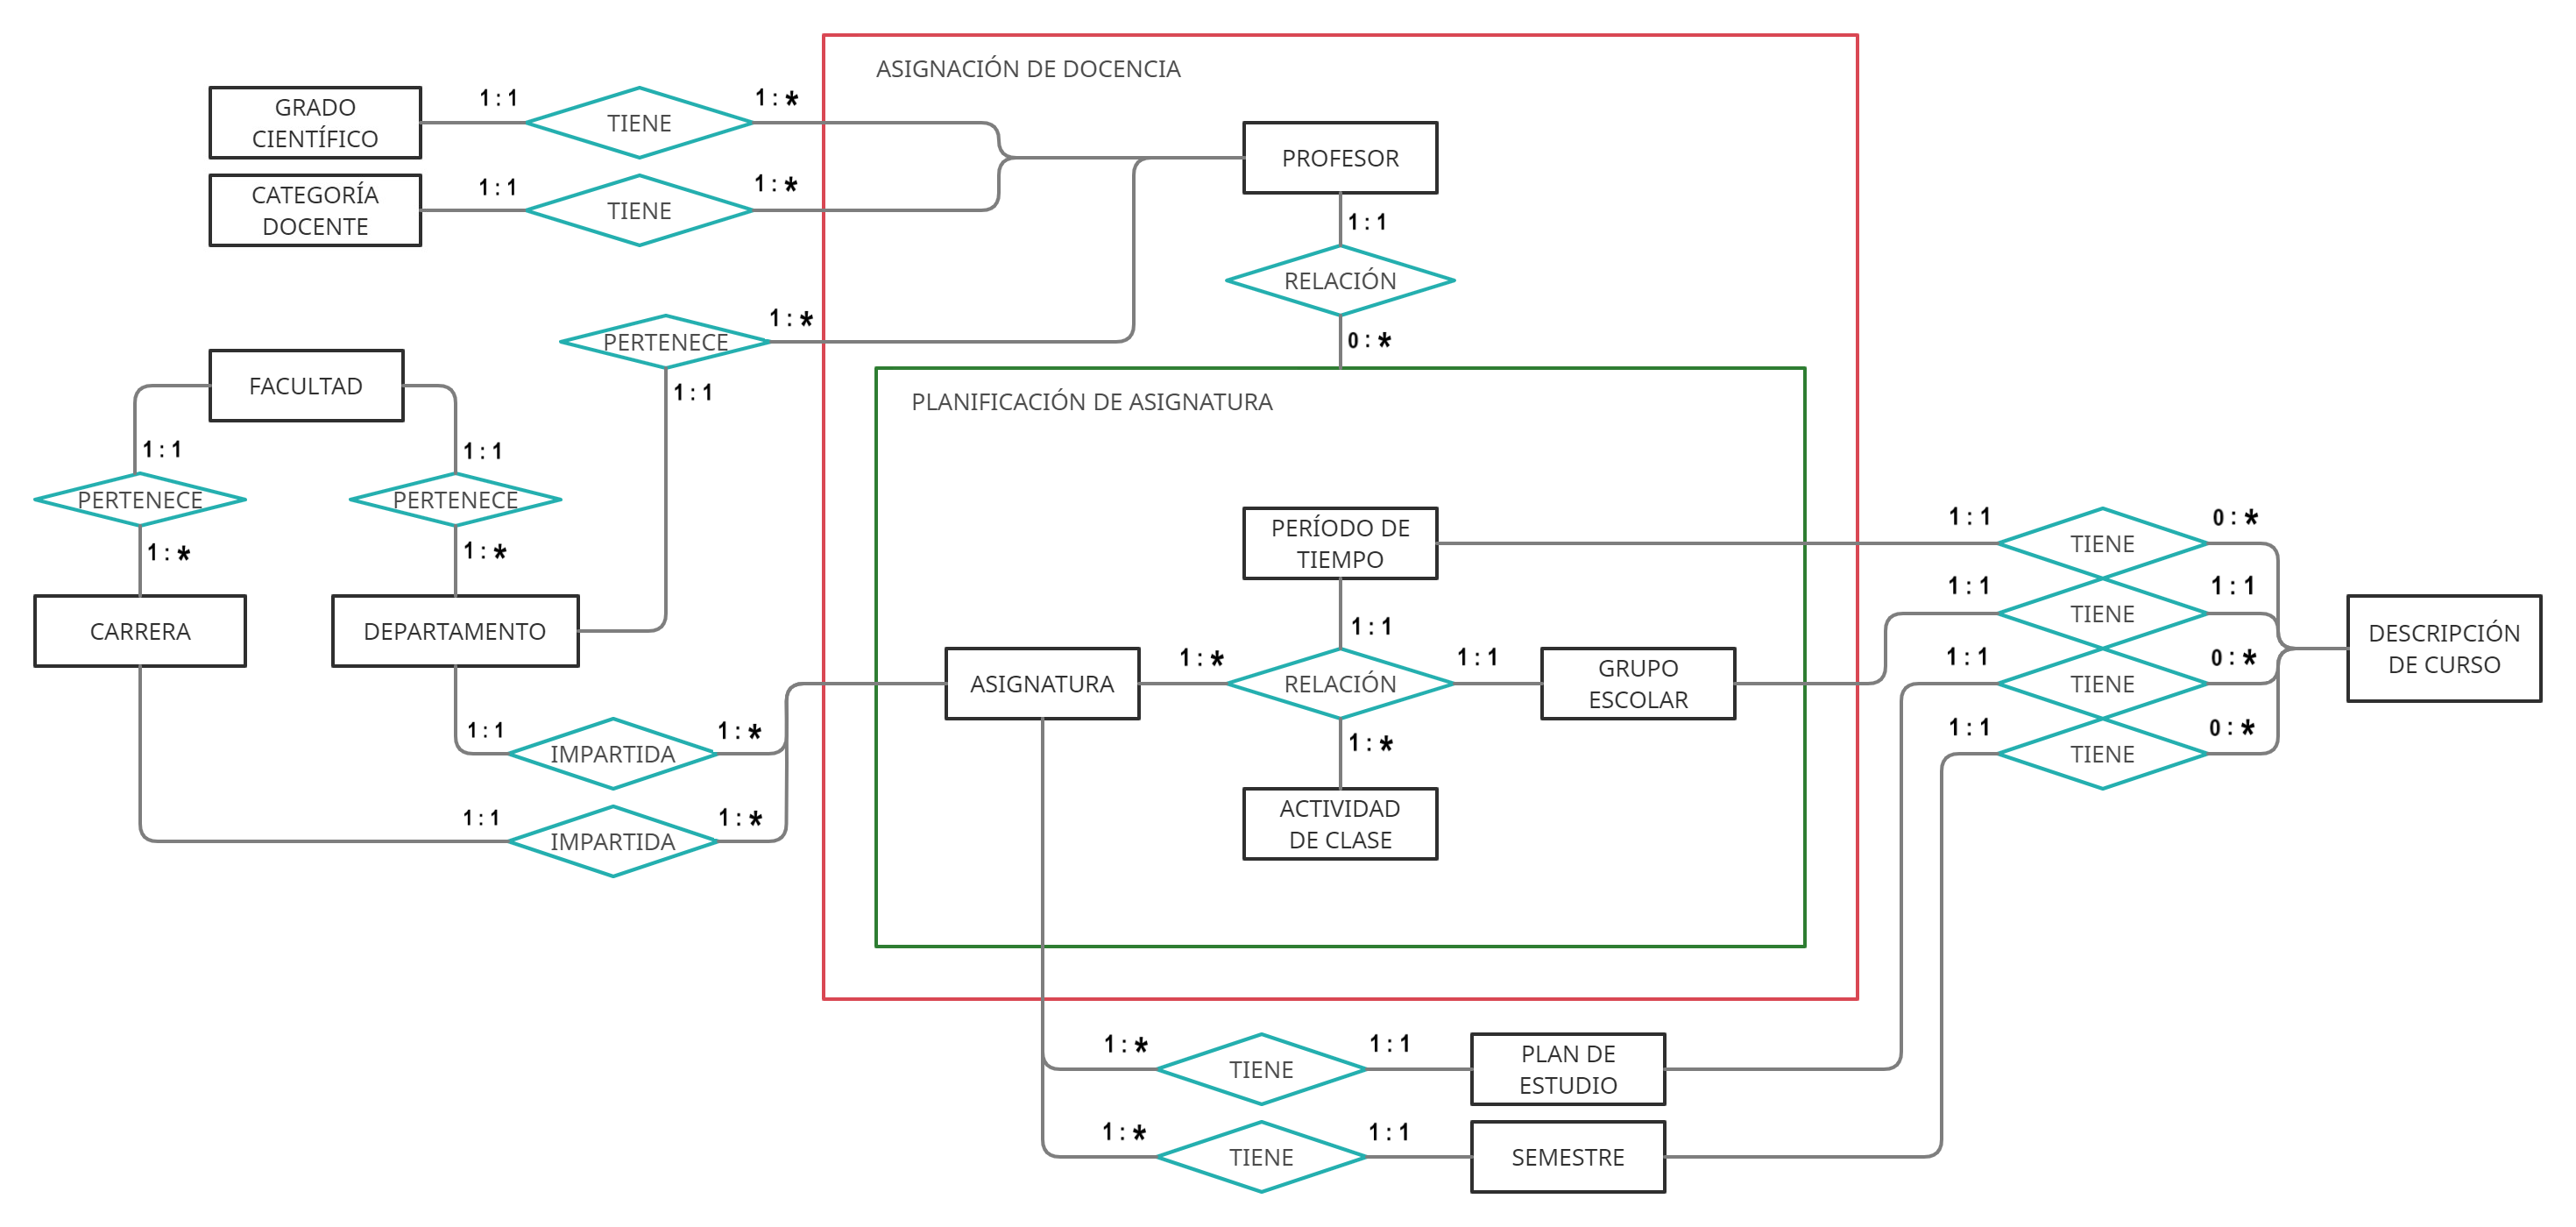
\includegraphics[scale=0.2]{Graphics/Database/MERXX-TA-FINAL.png}
\end{figure}


Con el objetivo de simplificar la representación del modelo entidad-relación
no se agregaron a la imagen los atributos correspondientes a cada entidad, por lo 
que a continuación se describen las entidades en mayor profundidad.


\subparagraph{FACULTAD:}
Representa las facultades de la Universidad de La Habana.
El nombre de la facultad se modela como un atributo, mientras que 
las carreras que se estudian en la facultad y los departamentos que pertenecen 
a ella, se modelan como relaciones con las entidades CARRERA y DEPARTAMENTO, respectivamente.
Una facultad tiene uno o muchos departamentos, y en 
una facultad se pueden estudiar una o más carreras.

\subparagraph{CARRERA:}
Representa las carreras que se estudian en la Universidad de La Habana.
El nombre de la carrera se modela como un atributo, mientras que la facultad a la que pertenece la carrera y
las asignaturas que se imparten en ella, se modelan como relaciones con las entidades FACULTAD y
ASIGNATURA, respectivamente. 
Una carrera pertenece a una única facultad y en una carrera se imparten una o muchas asignaturas.

\subparagraph{DEPARTAMENTO:}
Representa los departamentos de una facultad de la Universidad de La Habana.
El nombre del departamento se modela como un atributo, mientras que los profesores que 
pertenecen a un departamento, las asignatura que son atendidas por el departamento y la 
facultad a la que pertenece el departamento, se modelan como relaciones con las entidades 
PROFESOR, FACULTAD y ASIGNATURA, respectivamente. Un departamento pertenece a una única facultad,
un departamento atiende una o muchas asignaturas y a un departamento pertenecen uno o muchos 
profesores.

\subparagraph{PROFESOR:}
Agrupa los datos asociados a los profesores.
Los campos nombre y apellidos se modelan como atributos,  
mientras que, la categoría docente, el grado 
científico de un profesor y el departamento al que pertenece, se modelan como 
relaciones con las entidades CATEGORÍA DOCENTE, GRADO CIENTÍFICO y 
DEPARTAMENTO, respectivamente. Un profesor pertenece a un único departamento y puede tener solo 
un grado científico y una categoría docente. 


\subparagraph{CATEGORÍA DOCENTE:}
Representa la categoría docente que tienen los profesores.
El nombre de la categoría docente se modela como un atributo. 
Pueden existir uno o muchos profesores con una misma categoría docente.

\subparagraph{GRADO CIENTÍFICO:}
Representa el grado científico que tienen los profesores.
El nombre del grado científico se modela como un atributo.
Pueden existir uno o muchos profesores con un mismo grado científico.





\subparagraph{ASIGNATURA:}
Agrupa los datos asociados a las asignaturas.
Los campos nombre de la asignatura y cantidad de horas 
totales a impartir, se modelan como atributos, mientras que
el plan de estudio asociado a la asignatura, el semestre en el que se 
imparte, el departamento responsable de la asignatura y la carrera a la 
que pertenece, se modelan como relaciones con las entidades
PLAN DE ESTUDIO, SEMESTRE, DEPARTAMENTO y CARRERA respectivamente. Una asignatura 
es atendida por un único departamento, pertenece a una única carrera, se imparte en un 
único semestre y tiene un único plan de estudio. Las asignaturas que se imparten de forma 
anual son representadas como dos asignaturas independientes.

\subparagraph{PLAN DE ESTUDIO:}
Representa el plan de estudio por el que se rige una asignatura.
El nombre del plan de estudio se modela como un atributo.
Pueden existir una o muchas asignaturas con el mismo plan de estudio.



\subparagraph{SEMESTRE:}
Representa los semestres asociados a una carrera. 
El nombre del semestre se modela como un atributo.
Pueden existir una o muchas asignaturas que se imparten en 
el mismo semestre. 


\subparagraph{PERÍODO DE TIEMPO:}
Representa los períodos de tiempo del año.
El nombre del período de tiempo se modela como un atributo.
Pueden existir una o muchas asignaturas que se imparten en 
el mismo período de tiempo.


\subparagraph{GRUPO ESCOLAR:}
Representa los años académicos asociados a una carrera, como por ejemplo:
Matemática primer año (M1) o Computación tercer año (C3).
El nombre del grupo escolar se modela como un atributo.

\subparagraph{ACTIVIDAD DE CLASE:}
Representa los tipos de actividades que se imparten en una asignatura, 
tales como: conferencias, clases prácticas, seminarios, laboratorios, otros. 

\subparagraph{PLANIFICACIÓN DE ASIGNATURA:}
Se crea con el objetivo de modelar la separación de una asignatura
según las actividades de clases a impartir, en un período de tiempo y para
un grupo escolar específico. Está compuesta por la agregación de las entidades ASIGNATURA, ACTIVIDAD DE CLASE, GRUPO 
ESCOLAR y PERÍODO DE TIEMPO.
Se agregan los atributos cantidad de horas para el tipo de actividad a realizar y 
la cantidad de grupos.
Por ejemplo (poner ejemplo real de una asignatura
con distintas act de clase y como queda la separación)



% Entidad creada con el objetivo de separar las distintas actividades 
% que se imparten en una asignatura ( conferencia, clases 
% prácticas, seminarios, laboratorios, otras )  para
% realizar la asignación de docencia. Cuenta con una ASIGNATURA,
% en un PERÍODO DE TIEMPO, con el tipo de ACTIVIDAD DE CLASE y 
% el GRUPO ESCOLAR correspondiente. Por ejemplo, una planificación de
% asignatura pudiera ser (Poner ejemplo real). 
% se hace necesaria 
% la separación de una ASIGNATURA en más de una instancia para representar 
% el tipo de actividad de clase ( conferencia, clases 
% prácticas, seminarios, laboratorios, otras ), que va a recibir un 
% grupo escolar, en un período de tiempo.



\subparagraph{ASIGNACIÓN DE DOCENCIA:}
Representa las asignaciones de planificaciones de asignaturas a profesores.
Además se agrega un atributo porciento que indica el porcentaje del total de horas 
a impartir que asume el profesor asignado. Un profesor puede 
tener asignada cero o muchas planificaciones de asignaturas y una planificación de 
asignatura puede estar asignada a uno o muchos profesores.


\subparagraph{DESCRIPCIÓN DE CURSO:}
Representa el grupo escolar vigente en el curso actual. Está 
compuesta por la agregación de las entidades GRUPO ESCOLAR,
PERÍODO DE TIEMPO, PLAN DE ESTUDIO y SEMESTRE.  
Por ejemplo, una DESCRIPCIÓN DE CURSO puede ser 
que el grupo escolar C4 (Computación de cuarto año), con plan de
estudio E, se encuentra en el semestre 8,  en el período de tiempo septiembre-diciembre.






\section{Modelación de los tribunales de tesis}
Para la modelación del proceso de confección de los tribunales de tesis,
se crea un esquema basado en el modelo entidad-relacional extendido como en el 
proceso anterior. 


\begin{figure}[H]
    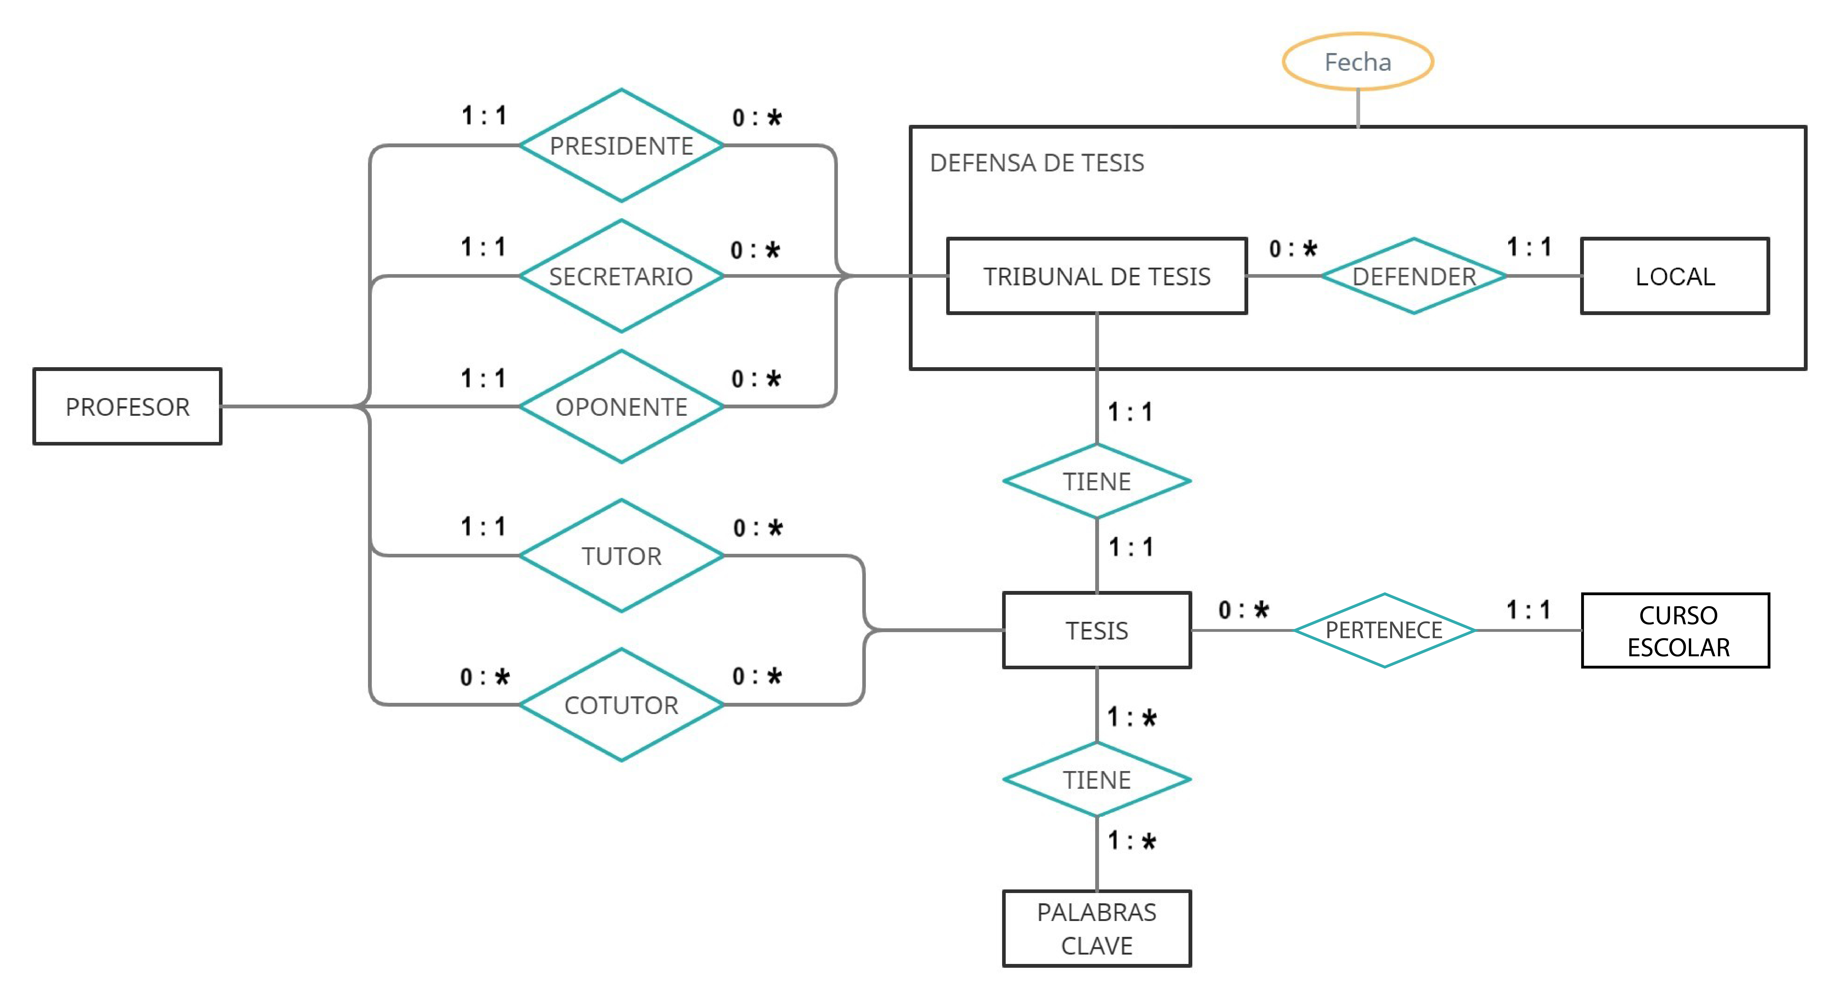
\includegraphics[scale=0.22]{Graphics/Database/MERXX-TC-FINAL.png}
\end{figure}


\subparagraph{TESIS:}
Agrupa los datos asociados a una tesis.
El título de la tesis y el autor se modelan como atributos, mientras que
el tutor, los cotutores y las palabras claves se modelan como relaciones con 
las entidades PROFESOR (tutor y cotutores) y PALABRAS CLAVES.
Una tesis tiene un único tutor, puede tener cero o muchos cotutores y tiene 
una o muchas palabras claves. 

\subparagraph{PALABRAS CLAVES:}
Representa las palabras claves que describen el contenido de una tesis.
El nombre o texto de las palabras claves se modela como un atributo. Una 
palabra clave puede aparecer en una o muchas tesis. 


\subparagraph{TRIBUNAL DE TESIS:}
Representa el tribunal de la defensa de una tesis.
Está compuesto por los miembros del tribunal: presidente, secretario y oponente, 
y la tesis, campos que se modelan como relaciones con las entidades PROFESOR y TESIS, respectivamente.
Un tribunal de tesis tiene una única tesis, un único presidente, un único secretario y 
un único oponente.


\subparagraph{DEFENSA DE TESIS:}
Representa el acto de defensa de la tesis. 
Está compuesta por un tribunal de tesis, en un local y una 
fecha determinada. La fecha se modela como un atributo mientras que 
el tribunal y el local se modelan como relaciones con las entidades TRIBUNAL DE 
TESIS y LOCAL, respectivamente. Una defensa de tesis tiene un único tribunal de tesis,
una única fecha y un único local.



\subparagraph{LOCAL:}
Representa el local donde se lleva a cabo la defensa de las tesis.
El nombre del local se modela como un atributo. 
En un local se puede realizar la defensa de cero o muchas tesis.


\subparagraph{PROFESOR:}
Se utiliza la misma entidad creada en el proceso de asignación de docencia.
Un profesor puede tener el rol de presidente, secretario u oponente en cero o 
muchos tribunales de tesis. Un profesor puede ser 
tutor o cotutor de cero o muchas tesis. \\


DESPUES DE LA MODELACION DE CADA PROCESO CREO Q DEBO HABLAR UN 
POCO DEL PROCESO DE NORMALIZACION PARA ESOS ESQUEMAS, Y REVISAR SI 
ESTAN EN 3FN... 

NO SE QUE MAS MENCIONAR EN ESTE CAPITULO.


